\documentclass[a4paper, 12pt]{article}

\usepackage[table,xcdraw]{xcolor}
\usepackage{enumerate}
\usepackage{graphicx}
\usepackage[T5]{fontenc}
\usepackage[utf8]{inputenc}
\usepackage[margin = 2cm]{geometry}
\usepackage{amsfonts, amsmath, amssymb}
\usepackage[none]{hyphenat}
\usepackage{fancyhdr}
\usepackage{float}
\usepackage{hyperref}
\usepackage{caption}
\usepackage[nottoc, notlot, notlof]{tocbibind}

% for code section
\usepackage{listings}

% for sub-figure
\usepackage{subcaption}
% \usepackage{rotating}
% \usepackage{tikz}

\captionsetup[table]{skip=5pt}
\pagestyle{fancy}
\fancyhead[L]{Trường Đại học Khoa học Tự nhiên - ĐHQG TP.HCM}
\fancyhead[R]{Nhóm 17}

\begin{document}

\begin{titlepage}
    \begin{center}
        \vspace*{1cm}
        \Large\textbf{Đại học Quốc gia TP. HCM\\Trường Đại học Khoa học Tự nhiên}\\

        \vfill
        \line(1,0){450}\\[4mm]
        \LARGE\textbf{\MakeUppercase{Báo cáo Lab 03\\ Trực quan hóa dữ liệu với Tableau}}\\[3mm]
        \Large{Trực quan hoá dữ liệu (CSC10108)}\\[3mm]
        \Large{Nhóm 17}
        \line(1,0){430}\\
        \vfill

        \vfill
        TP Hồ Chí Minh, ngày 14/06/2021
    \end{center}
\end{titlepage}

\tableofcontents
\thispagestyle{empty}
\clearpage

\section{Thông tin nhóm}
    \begin{table}[H]
        \begin{tabular}{|c|c|l|c|c|}
        \hline
        STT & MSSV     & \multicolumn{1}{c|}{Họ tên} & Email                         & SĐT        \\ \hline
        1   & 18120078 & Ngô Phù Hữu Đại Sơn         & 18120078@student.hcmus.edu.vn & 0919070940 \\ \hline
        2   & 18120201 & Nguyễn Bảo Long             & 18120201@student.hcmus.edu.vn & 0981850699 \\ \hline
        3   & 18120227 & Phạm Văn Minh Phương             & 18120227@student.hcmus.edu.vn & 0343049359 \\ \hline
        4   & 18120253 & Mai Ngọc Tú             & 18120253@student.hcmus.edu.vn & 0981850699 \\ \hline
        5   & 1712424 & Hàn Văn Gia Hiên            & 1712424@student.hcmus.edu.vn & 0911572108 \\ \hline
        \end{tabular}
        \caption{Bảng danh sách thành viên nhóm}
    \end{table}
    \clearpage

    \section{Phân tích hoàn thiện yêu cầu}

    \subsection{Tổng quan mức độ hoàn thành mỗi yêu cầu}

    \begin{table}[H]
        \begin{tabular}{|c|l|l|c|}
        \hline
        STT & \multicolumn{1}{c|}{Yêu cầu} & \multicolumn{1}{c|}{Công việc}                                                & Hoàn thành (\%) \\ \hline
        1 & Analysis of Car MPG data      & \begin{tabular}[c]{@{}l@{}}- Trả lời câu hỏi\\ - Vẽ biểu đồ và nghiên cứu lịch sử\end{tabular}              & 100/100\\ \hline
        2 & Story of EPC data & \begin{tabular}[c]{@{}l@{}}- Trực quan các biến, vẽ biểu đồ \\giải thích ý nghĩa, viết story\end{tabular}                          & 100/100 \\ \hline\end{tabular}
        \caption{Bảng phân tích hoàn thành yêu cầu}
    \end{table}

    \subsection{Mức độ hoàn thành của thành viên nhóm}

        \begin{table}[]
            \begin{tabular}{|c|l|l|c|}
            \hline
            STT & \multicolumn{1}{c|}{Họ tên} & \multicolumn{1}{c|}{Công việc tham gia}                                                                                                            & Hoàn thành (\%) \\ \hline
            1   & Ngô Phù Hữu Đại Sơn         & - Vẽ biểu đồ cho phần Story of EPC data                                                                                                            & 100/100         \\ \hline
            2   & Nguyễn Bảo Long             & \begin{tabular}[c]{@{}l@{}}- Vẽ biểu đồ câu hỏi 4, 5, 6 phần \\ Exploratory analysis of Car MPG data\\ Nhận xét biểu đồ\end{tabular}               & 100/100         \\ \hline
            5   & Phạm Văn Minh Phương        & \begin{tabular}[c]{@{}l@{}}- Tìm hiểu lịch sử xe hơi giải thích dữ liệu \\ phần Exploratory analysis of Car MPG data\\ - Viết báo cáo\end{tabular} & 100/100         \\ \hline
            5   & Mai Ngọc Tú                 & \begin{tabular}[c]{@{}l@{}}- Vẽ biểu đồ câu hỏi 1, 2, 3 phần \\ Exploratory analysis of Car MPG data\\ - Nhận xét biểu đồ\end{tabular}             & 100/100         \\ \hline
            5   & Hàn Văn Gia Hiên            & \begin{tabular}[c]{@{}l@{}}- Vẽ biểu đồ câu hỏi 7, 8, 9 phần \\ Exploratory analysis of Car MPG data\\ - Nhận xét biểu đồ\end{tabular}             & 100/100         \\ \hline
            \end{tabular}
        \end{table}
    \clearpage

\section{Exploratory analysis of Car MPG data}

\subsection{Trả lời câu hỏi}
    \subsubsection{Có bao nhiêu xe và bao nhiêu thuộc tính trong bộ dữ liệu}
        \begin{itemize}
            \item Có 312 xe và 9 thuộc tính trong bộ dữ liệu
        \end{itemize}

    \subsubsection{Có bao nhiêu công ty xe hơi riêng biệt xuất hiện trong bộ dữ liệu? Tên của chiếc xe có MPG cao nhất là gì? Công ty nào sản xuát nhiều xe 8 xi-lanh nhất? Tên của những chiếc xe 3 xi-lanh? Tìm kiếm trên internet thông tin về lịch sử và độ phổ biến của những chiếc xe 3 xi-lanh này.}
        \begin{itemize}
            \item Có 38 công ty xe hơi xuất hiện trong bộ dữ liệu
            \item Xe có MPG cao nhất: Mazda glc
            \item Công ty sản xuất nhiều xe 8 xi-lanh nhất: Ford
            \item Tên những xe có 3 xi lanh: Mazda rx2 coupe, Maxda rx3, Mazda rx-4, Mazda rx-7 gs
            \item Lịch sử và độ phổ biến của những chiếc xe 3 xi-lanh trên:
                \begin{itemize}
                    \item Mazda RX-2 là một chiếc ô tô cỡ vừa ra mắt vào năm 1970 và được sản xuất tới năm 1979. Mazda RX-2 được định hướng là một chiếc ô tô cho gia đình và sử dụng động cơ quay. Là một phiên bản cực kì thành công và có độ phổ biến rất cao tại thời điểm đó.
                    \item Mazda RX3 được bán từ năm 1971 tới năm 1978. Vào năm đầu ra mắt, doanh số toàn cầu của RX-3 là khoảng 200,000 chiếc. Từ 1972 trở đi, doanh số RX-3 đã vượt hẳn RX-2 và đạt kỉ lục bán ra 105,819 chiếc chỉ trong năm 1972, giúp tổng xe động cơ xoay đạt 500,000 chiếc. Từ 1974 trở đi doanh số của RX-4 cao hơn nhưng RX-3 vẫn được các tay đua tin dùng trong các giải đua xe chuyên nghiệp
                    \item Mazda RX-4 là mẫu xe điều hành được sản xuất tại Nhật từ 1966 tới 1991. Được marketing là một chiếc xe thể thao sang trọng.
                    \item Mazda RX-7 là mẫu xe thể thao được sản xuất từ năm 1978 tới 2002. Là dòng xe động cơ quay bán chạy số 1 mọi thời đại với 811,634 chiếc được bán ra. 
                \end{itemize}
        \end{itemize}
        
    \subsubsection{Khoảng, trung bình, độ lệch chuẩn của từng thuộc tính? Chú ý tới những giá trị tiềm ẩn còn thiếu.}
        \begin{table}[H]
        \centering
        \begin{tabular}{l|l|l|l|l|}
        \cline{2-5}
                                    & mpg       & cyclinder & displacement & horsepower \\ \hline
        \multicolumn{1}{|l|}{Range} & 37.6      & 5         & 387          & 184        \\ \hline
        \multicolumn{1}{|l|}{Mean}  & 23.504433 & 5.475369  & 194.779557   & 105.081281 \\ \hline
        \multicolumn{1}{|l|}{STD}   & 7.738736  & 1.712160  & 104.922458   & 38.480533  \\ \hline
        \end{tabular}
        \end{table}
        
        \begin{table}[H]
        \centering
        \begin{tabular}{l|l|l|l|l|}
        \cline{2-5}
                                    & weight      & acceleration & model     & origin   \\ \hline
        \multicolumn{1}{|l|}{Range} & 3527        & 16.8         & 12        & 2        \\ \hline
        \multicolumn{1}{|l|}{Mean}  & 2979.413793 & 15.519704    & 75.921182 & 1.568966 \\ \hline
        \multicolumn{1}{|l|}{STD}   & 847.004328  & 2.803359     & 3.748737  & 0.797479 \\ \hline
        \end{tabular}
        \end{table}
        
    \subsubsection{Vẽ histogram cho từng thuộc tính. Chú ý việc chọn số lượng bin phù hợp. Viết 2-3 câu tóm tắt những khía cạnh thú vị trong dữ liệu bằng cách nhìn vào histogram}
        \begin{figure}[H]
            \centering
                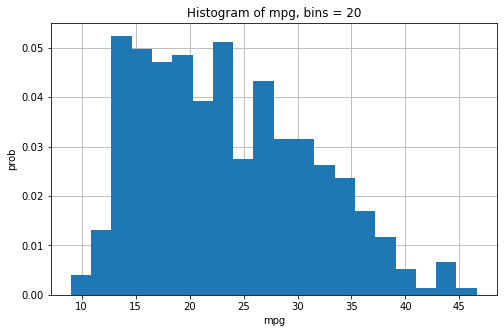
\includegraphics[scale=0.9]{img/mpg.png}
                \caption{Histogram của mpg}
        \end{figure}
        
        \begin{figure}[H]
            \centering
                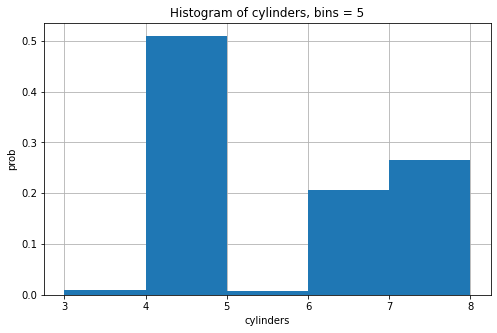
\includegraphics[scale=0.9]{img/cylinders.png}
                \caption{Histogram của cylinders}
        \end{figure}
        
        \begin{figure}[H]
            \centering
                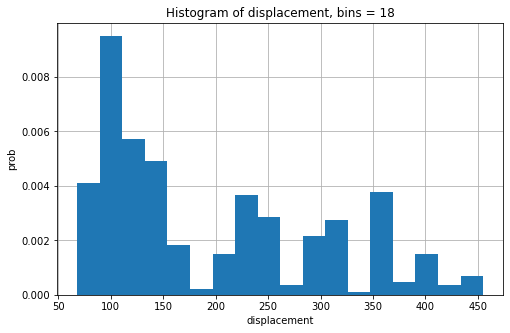
\includegraphics[scale=0.9]{img/displacement.png}
                \caption{Histogram của displacement}
        \end{figure}
        
        \begin{figure}[H]
            \centering
                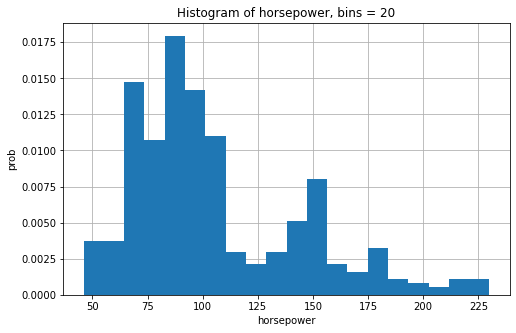
\includegraphics[scale=0.9]{img/horsepower.png}
                \caption{Histogram của horsepower}
        \end{figure}
        
        \begin{figure}[H]
            \centering
                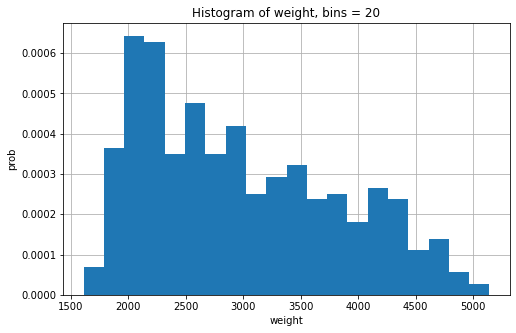
\includegraphics[scale=0.9]{img/weight.png}
                \caption{Histogram của weight}
        \end{figure}
    
        \begin{figure}[H]
            \centering
                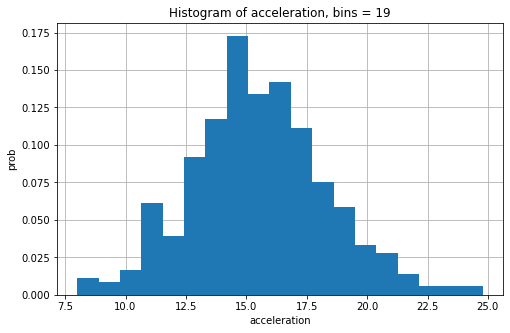
\includegraphics[scale=0.9]{img/acceleration.png}
                \caption{Histogram của acceleration}
        \end{figure}
        
        \begin{figure}[H]
            \centering
                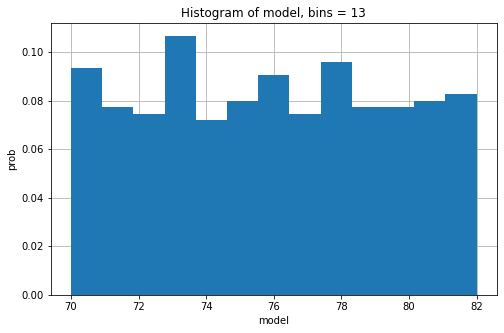
\includegraphics[scale=0.9]{img/model.png}
                \caption{Histogram của model}
        \end{figure}
        
        \begin{figure}[H]
            \centering
                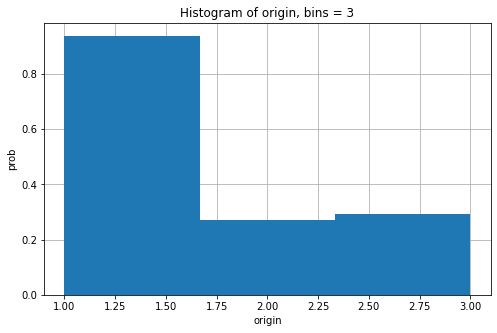
\includegraphics[scale=0.9]{img/origin.png}
                \caption{Histogram của origin}
        \end{figure}
        
        \begin{itemize}
            \item Biểu đồ histogram cung cấp cái nhìn tổng quát về phân bố dữ liệu
            \item Các khía cạnh rút ra được từ histogram:
                \begin{itemize}
                    \item `model` của các hãng xe được sản suất khá đồng đều, trung bình mỗi năm, các hãng đều có ra mẫu xe mới. Trong đó, năm 1973 cho ra đời nhiều mẫu xe nhất
                    \item Số lượng xi-lanh phổ biến nhất là 4, kế đến là 7 và 6
                    \item Thông thường, với 1 gallon nhiên liệu, 1 xe có thể đi được từ 12 đến 25 dặm
                \end{itemize}
        \end{itemize}
    
    \subsubsection{Vẽ scatterplot của thuộc tính weight với MPG. Có kết luận gì về quan hệ giữa hai thuộc tính này? Hệ số tương quan giữa hai thuộc tính là bao nhiêu?}
        \begin{figure}[H]
            \centering
                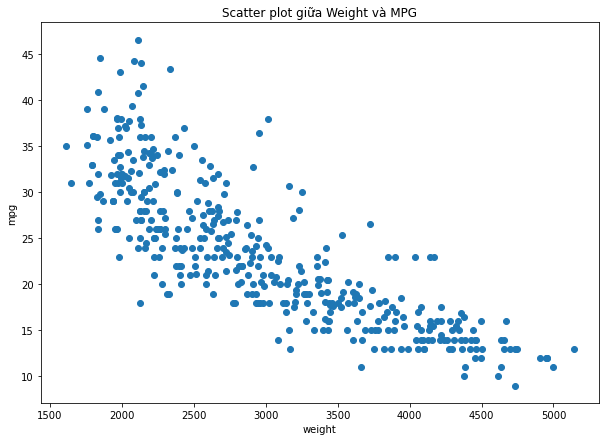
\includegraphics[scale=0.8]{img/weight-mpg.png}
                \caption{Scatter plot giữa weight và MPG}
        \end{figure}
        
        \begin{itemize}
            \item Hệ số tương quan rất cao và âm chứng tỏ giữa 2 thuộc tính này tồn tại quan hệ nghịch biến
            \item Điều này là dễ hiểu vì khi tăng khối lượng xe và giữ nguyên lượng xăng thì xe sẽ phải tốn nhiều năng lượng hơn để di chuyển dẫn tới MPG (Số dặm đi được theo mỗi đơn vị nhiên liệu gallon) giảm.
        \end{itemize}
    \subsubsection{Vẽ scatterplot của thuộc tính year với cylinders. Thêm mội lượng noise ngẫu nhiên nhỏ vào giá trị để làm scatterplot đẹp hơn. Có thể kết luận được gì? Thực hiện tìm kiếm trên internet về lịch sử của công nghiệp xe hơi trong thập niên 70 có thể giải thích được kết quả}
        \begin{figure}[H]
            \centering
                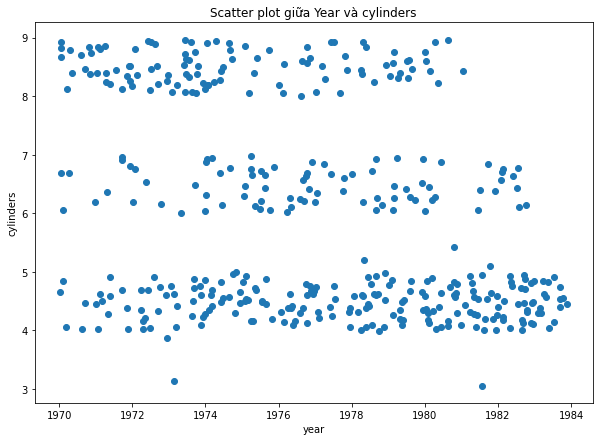
\includegraphics[scale=0.8]{img/year-cylinders.png}
                \caption{Scatter plot giữa year và cylinders}
        \end{figure}
        
        \begin{itemize}
            \item Việc bỏ thêm nhiễu vào dữ liệu giúp tăng hiệu suất trực quan (dễ quan sát được mật độ cũng như phân bố của dữ liệu)
            \item Ngoài ra, còn có thể dễ dàng xác định các điểm dữ liệu outlier
            \item Nhiều mẫu 8 xi lanh được sản xuất nhiều ở giai đoạn đầu những năm 70 (70-74) và giảm dần theo thời gian và biến mất hẳn vào các năm cuối
            \item Ngược lại, xe 4 xi lanh vẫn luôn là mẫu xe phổ biến nhất và được sản xuất ngày càng nhiều.
            \item Lịch sử công nghiệp xe hơi những năm 70: 
                \begin{itemize}
                    \item Khoảng thời gian đầu, mọi người đều thích sử dụng những chiếc xe có 8 xi lanh do đặc tính của nó: nhanh, mạnh, kiểu dáng đẹp, hầm hố. Đồng thời vào khoảng thời gian này, việc xe 8 xi-lanh thống trị ở các giải đua xe cũng góp phần định hướng thị trường xe hơi ngày đó.
                    \item Đây là khoảng thời gian mà thế giới xảy ra khủng hoảng dầu khí nên có rất nhiều đạo luật được ban hành (Emergency Petroleum Allocation Act - 1973; Energy Policy and Conservation Act - 1975...) , ảnh hưởng trực tiếp tới việc sản xuất công nghiệp. Ngoài ra, khoảng thời gian này cũng là lúc hàng loạt đạo luật về khí thải ra đời. Các hãng xe hơi buộc phải đưa ra giải pháp để giảm 2 thứ: nhiên liệu tiêu thụ và khí thải. Điều này dẫn tới kết quả hiển nhiên trong việc các hãng xe gia tăng việc sử dụng các động cơ 4 xi-lanh để chế tạo xe hơi vì chúng nhỏ hơn, nhẹ hơn và thân thiện môi trường hơn và công suất của chúng cũng phù hợp cho nhu cầu phổ thông. 
                    \item Cũng trong khoảng thời gian này, bộ tăng áp (turbocharger) cũng được sử dụng ngày càng phổ biến vì nó giúp những động cơ 4, 6 xi lanh có sức mạnh như những động cơ có 8 xi lanh nhưng vẫn giữ được kích cỡ nhỏ gọn và sử dụng ít nhiên liệu và xả ít khí thải hơn. Đột phá thực sử xảy ra vào năm 1978 khi động cơ diesel tăng áp đầu tiên được ra đời theo chiếc Mercedes Benz 300SD, theo sau là động cơ VW Golf Turbodiesel vào năm 1981. Động cơ tăng áp sử dụng diesel có hiệu suất cao hơn và xả thải ít hơn hẳn động cơ chạy bằng gas ở trên các mẫu xe trước đó
                    \item Các điểm outlier trên biểu đồ là bốn mẫu xe 3 xi lanh ra đời vào các năm 1972, 1973, 1977, 1980. Tất cả đều đến từ hãng xe Mazda vì họ muốn giữ sự khác biệt của mình với các hãng xe khác và loại động cơ xoay 3 xi-lanh mà họ sử dụng cũng có hiệu suất và lợi thế ổn định.
                \end{itemize}
        \end{itemize}
    
    \subsubsection{Thể hiện 2 scatterplot thú vị với bạn. Bàn luận về những gì bạn thấy}
        \begin{figure}[H]
            \centering
                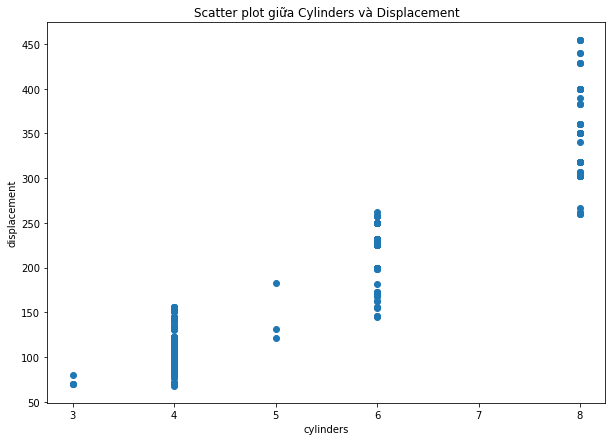
\includegraphics[scale=0.8]{img/cylinders-displacement.png}
                \caption{Scatter plot giữa  cylinders và displacement}
        \end{figure}
        
        \begin{itemize}
            \item Ta có thể quan sát rõ được sự tương quan thuận giữa số cylinder và displacement.
            \item Đúng như trong thực tế, những cỗ máy có nhiều xi-lanh thường đi với một dung tích lớn để tăng công suất cho xe.
            \item Động cơ 4 xi-lanh, dung tích nhỏ thường được sử dụng cho xe tầm trung, đa dụng nên có số lượng tương đối nhiều.
        \end{itemize}

        \begin{figure}[H]
            \centering
                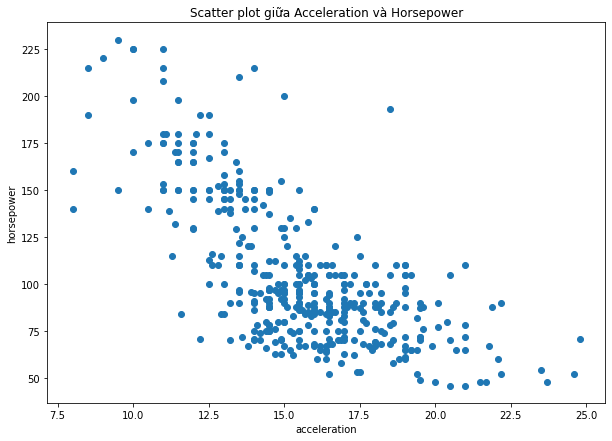
\includegraphics[scale=0.8]{img/acceleration-horsepower.png}
                \caption{Scatter plot giữa  acceleration và horsepower}
        \end{figure}
        
    \subsubsection{Vẽ biểu đồ thời gian cho tất cả các công ty chỉ ra số xe hơi họ giới thiệu mỗi năm. Bạn có thấy xu hướng nào thú vị không?}
        \begin{figure}[H]
            \centering
                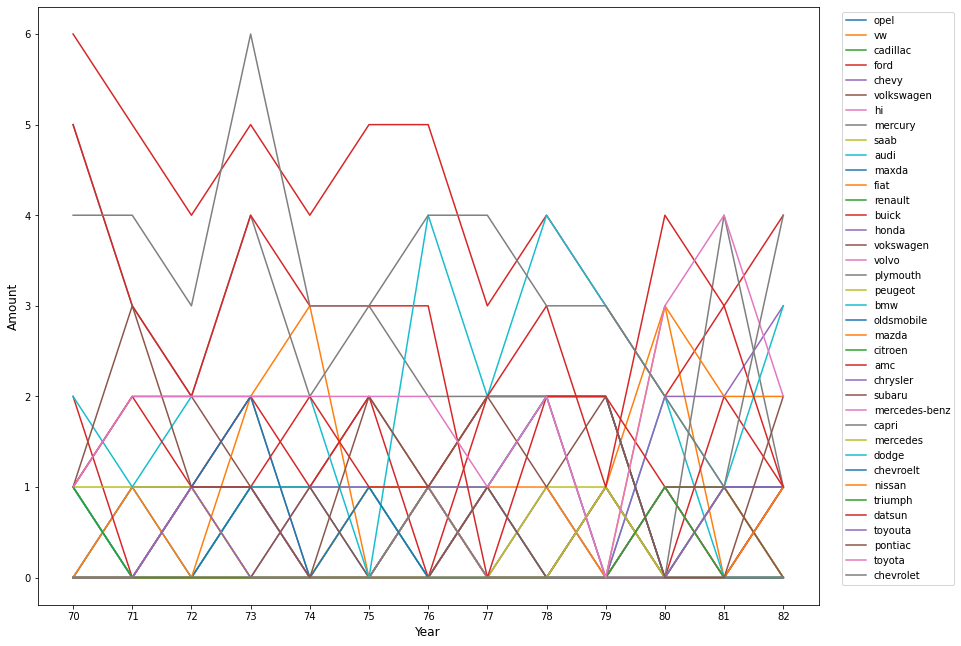
\includegraphics[scale=0.5]{img/timeseries.png}
                \caption{Scatter plot giữa  acceleration và horsepower}
        \end{figure}
        
        \begin{itemize}
            \item Các hãng lớn sẽ ra mắt từ 2 - 6 xe mỗi năm, còn các hãng còn lại thì chỉ từ 1 - 2 xe.
            \item Các hãng xe có xu hướng ra mắt giảm dần số lượng dần về những năm cuối thập kỷ và cho ra mắt hàng loạt số lượng xe mới vào nhứng năm đầu của thập kỷ kế tiếp.
        \end{itemize}

    \subsubsection{Tính toán tương quan theo cặp, và vẽ heatmap với Matplotlib. Bạn có thấy tuông quan nào thú vị không?}
        \begin{figure}[H]
            \centering
                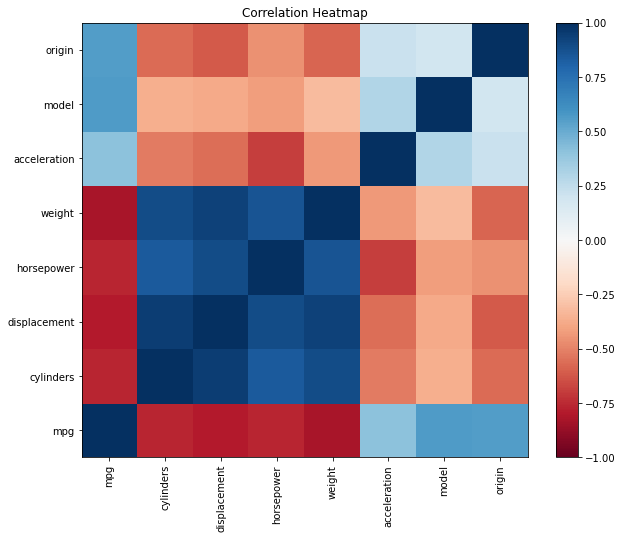
\includegraphics[scale=0.5]{img/heatmap.png}
                \caption{Heatmap thể hiện tương quan giữa các thuộc tính}
        \end{figure}
        
        \begin{itemize}
            \item Ta có thể thấy sự tương quan thuận cao giữa các thông số cơ khí với nhau (cylinders, displacement, horsepower, weight), những thông số này đại diện cho phân khúc, công suất của từng chiếc xe
            \item Thông số mpg tương quan nghịch cao với các thông số cơ khí trên thể hiện nếu xe càng mạnh, phân khúc càng cao thì sẽ càng tiêu hao nhiên liệu (mpg thấp).
            \item Thông số mpg tương quan thuận với model và origin thể hiện đời xe càng cao thì càng tiết kiệm nhiên liệu.
            \item Thông số acceleration tương quan nghịch với các thông số cơ khí trên thể hiện nếu xe càng to, công suất cao thì khả năng tăng tốc sẽ yếu.
        \end{itemize}
        
\clearpage
    
    \subsection{Story of Electric Power Compsumtion Data}
        \begin{figure}[H]
            \centering
            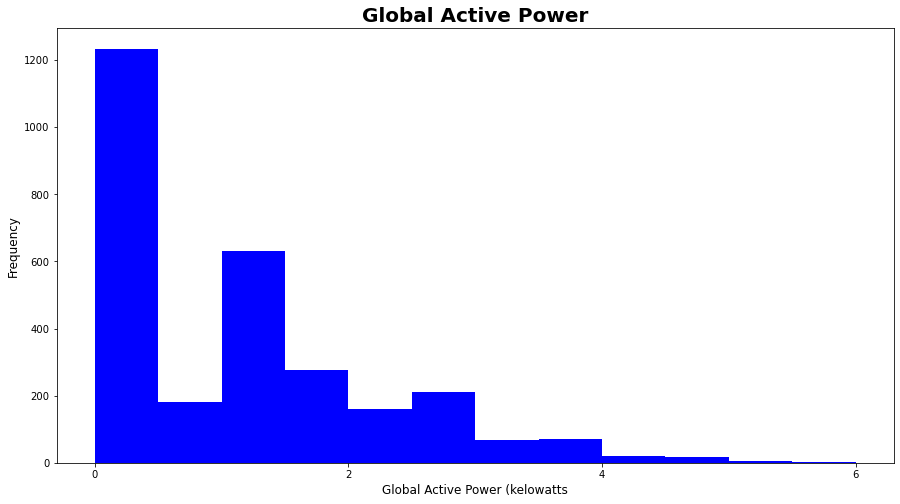
\includegraphics[scale=0.5]{img/GAP.png}
            \caption{Tần suất xuất hiện của các mức công suất}
        \end{figure}
        
        \begin{itemize}
            \item Hộ gia đình này sử dụng điện rất liên tục, luôn luôn có thiết bị điện được sử dụng trong nhà. Phần lớn thời gian sử dụng ở mức thấp (bật đèn...)
        \end{itemize}
        
        \begin{figure}[H]
            \centering
            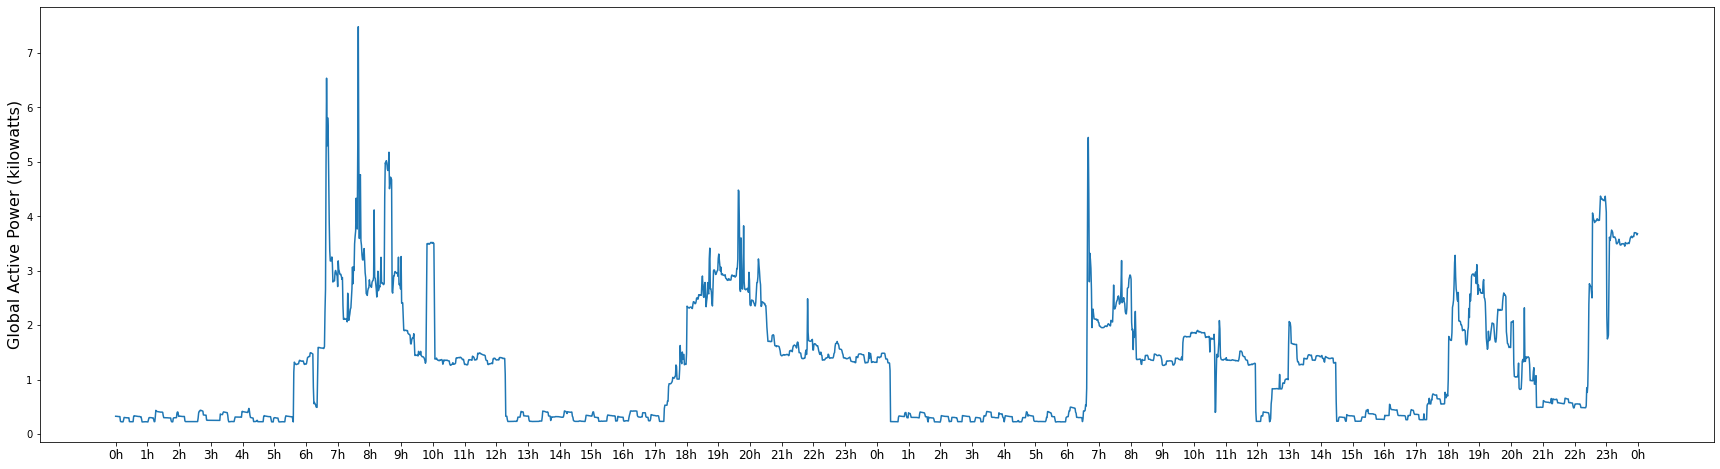
\includegraphics[scale=0.3]{img/GAP-hours.png}
            \caption{Mức công suất theo giờ}
        \end{figure}
        
        \begin{itemize}
            \item Hộ gia đình này có những khoảng sử dụng điện cao điểm. Cụ thể hơn là vào từ 6h - 12h và 17h-0h.
        \end{itemize}
        
        \begin{figure}[H]
            \centering
            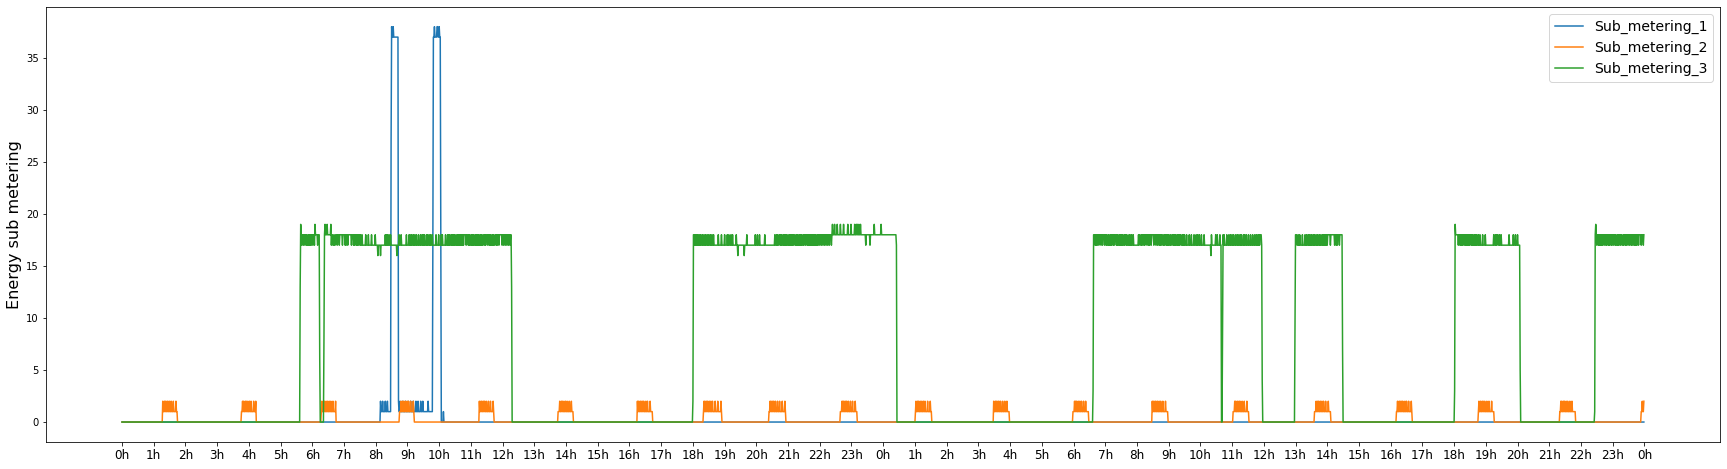
\includegraphics[scale=0.3]{img/meterings.png}
            \caption{Công đo được từ 3 điện kế}
        \end{figure}
        
        \begin{itemize}
            \item Có thể nhận biết rằng gia đình này đã nấu ăn vào khoảng 8h-10h ngày 01-02. Ở phòng bếp luôn có một chiếc tủ lạnh sử dụng điện theo chu kì theo chu kì 2 tiếng thì sẽ làm lạnh 30p. Máy sưởi và điều hòa được sử dụng khi trời sáng và khi đi ngủ, chỉ không sử dụng vào thời điểm trưa - chiều, khi trời ấm hơn.
        \end{itemize}
        
        \begin{figure}[H]
            \centering
            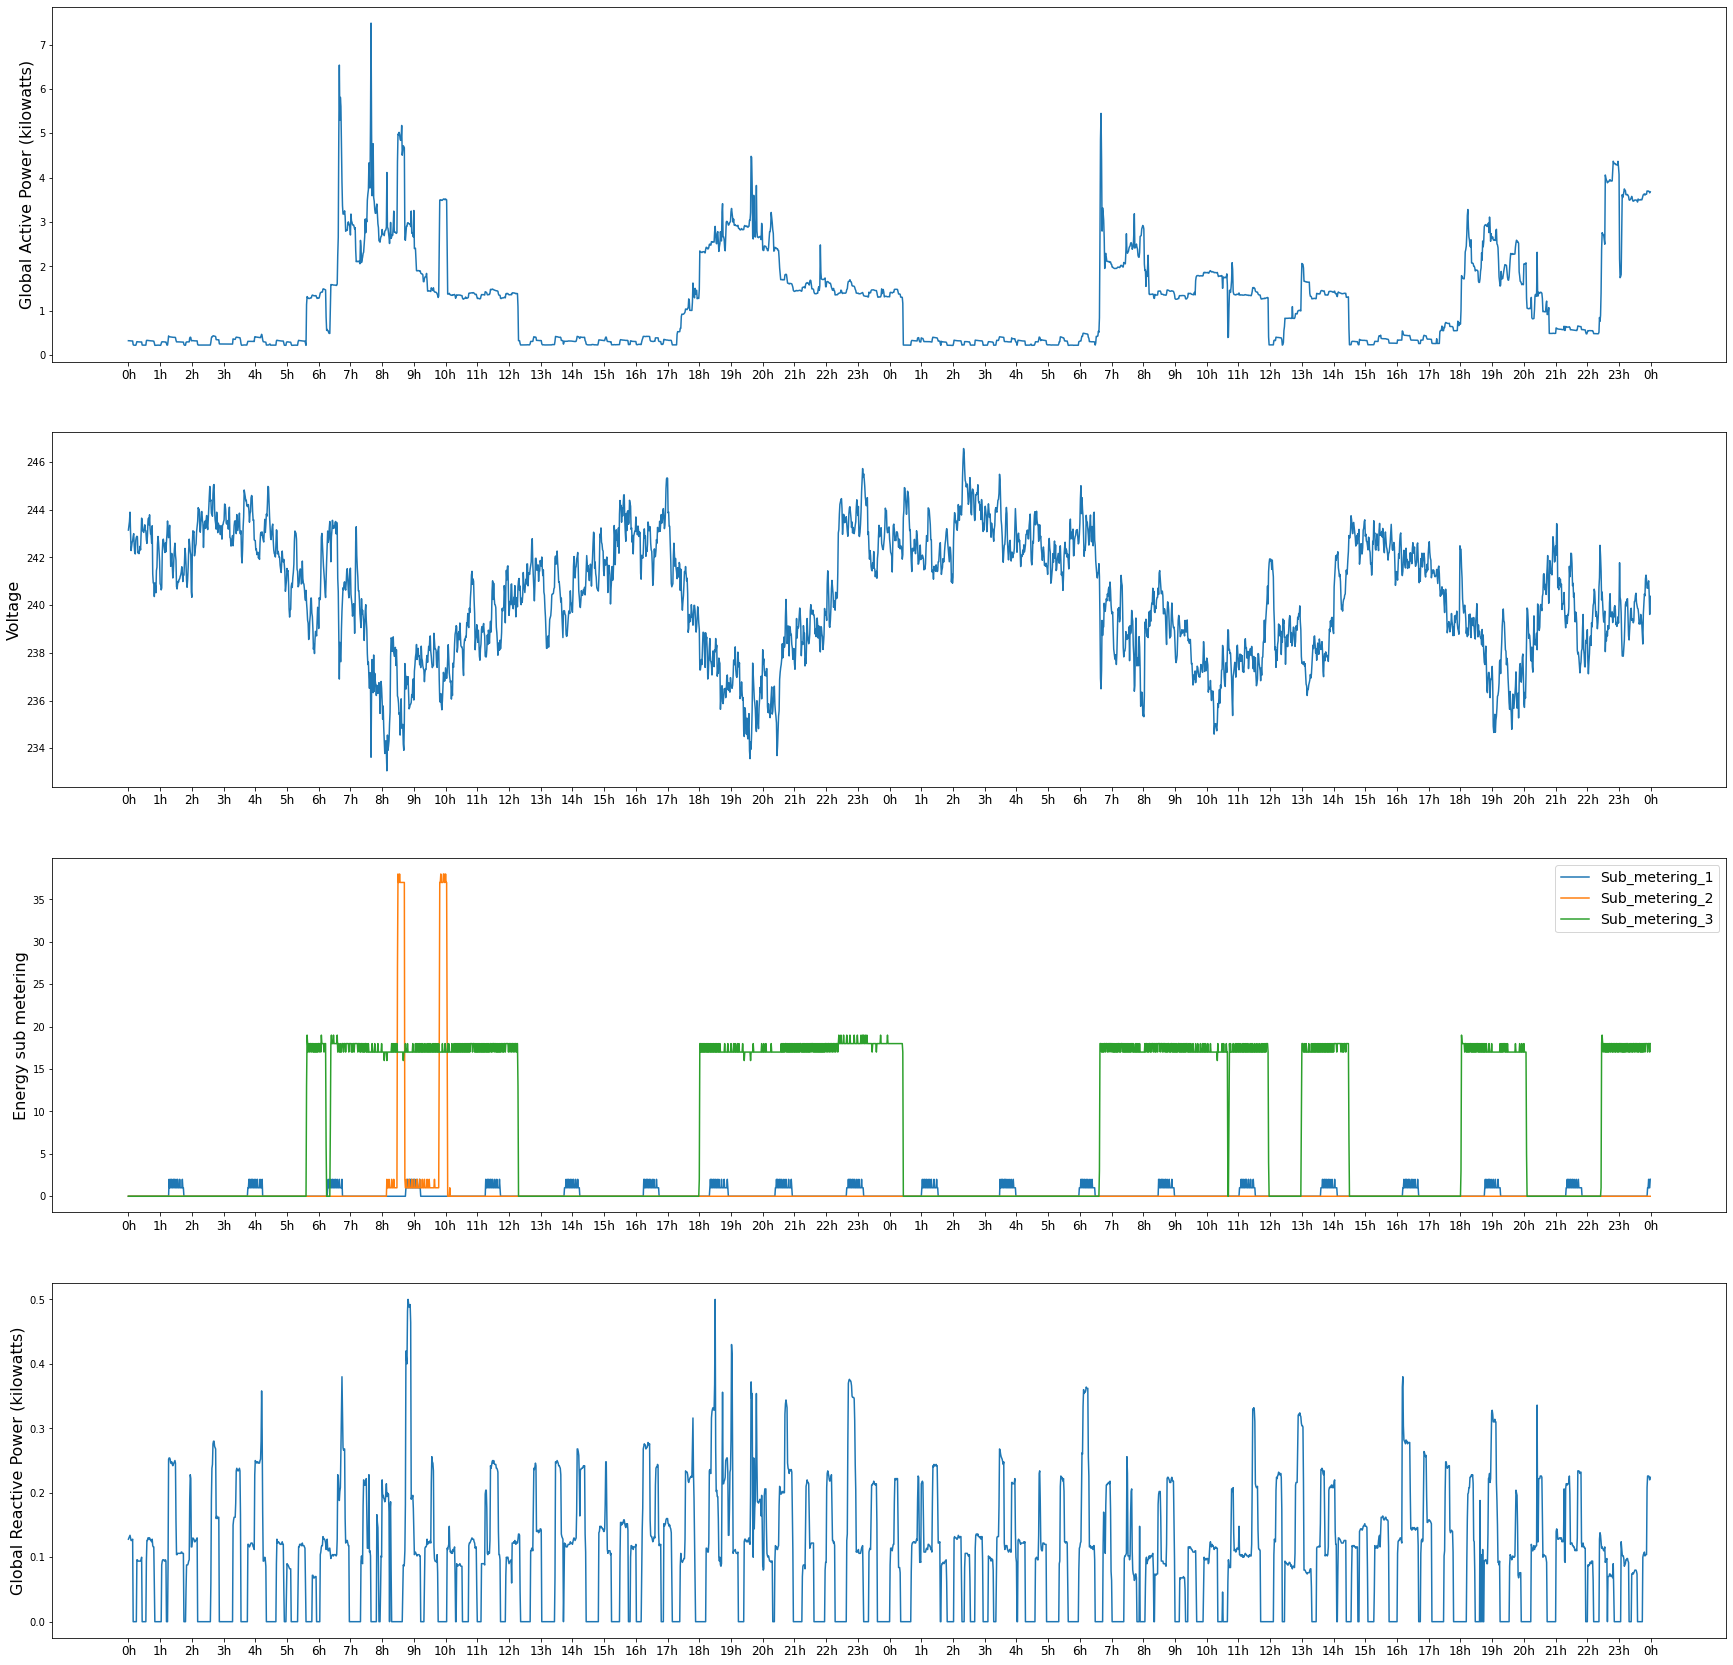
\includegraphics[scale=0.3]{img/all.png}
            \caption{Một số biểu đồ khác}
        \end{figure}
        
        \begin{itemize}
            \item Khảo sát các biểu đồ khác cũng cho thấy một số kết quả tương tự về khoảng giờ cao điểm. Hiệu điện thế sẽ giảm khi có nhiều thiết bị sử dụng điện. Mức công phản kháng cũng có sự tăng giảm đồng đều với mức công suất sử dụng.
        \end{itemize}

\clearpage

\section{Tham khảo}

    \begin{itemize}
        \item \url{https://classiccars.fandom.com/wiki/Mazda_RX-7}
        \item \url{https://classiccars.fandom.com/wiki/Mazda_RX-4}
        \item \url{https://en.wikipedia.org/wiki/Mazda_RX-7}
        \item \url{https://en.wikipedia.org/wiki/Mazda_Luce}
        \item \url{https://en.wikipedia.org/wiki/Mazda_Grand_Familia}
        \item \url{https://www.mazda.co.uk/why-mazda/news-and-events/mazda-news/articles/2021-50th-anniversary-of-the-mazda-rx-3/}
        \item \url{https://en.wikipedia.org/wiki/Mazda_Capella#RX-2}
        \item \url{http://www.turbos.bwauto.com/en/products/turbochargerHistory.aspx}
        \item \url{https://www.edmunds.com/car-reviews/features/the-history-of-the-mazda-3-a-look-back-through-time.html}
    \end{itemize}

\end{document}